\def\CTeXPreproc{Created by ctex v0.2.9, don't edit!}
%\documentclass{beamer}
\documentclass[%handout,
xcolor=pdftex]{beamer}
\mode<presentation> {
  \usetheme{Warsaw}
  \setbeamercovered{transparent}
}
\let\Tiny=\tiny
\usetheme{Singapore}
\usecolortheme{dolphin}
\usepackage{amsmath}
\usepackage{textcomp}
\usepackage{amssymb}
\usepackage{amsthm}
\usepackage{graphicx}
\usepackage{color}
\usepackage{lipsum}
\usepackage{hyperref}
\usepackage{multirow}
\usepackage{bm}
%\setbeamertemplate{headline}{}
\setbeamertemplate{footline}[page number]
\newcommand\Fontvi{\fontsize{9pt}{8}\selectfont}
\newcommand\Fontvii{\fontsize{7pt}{8}\selectfont}
\newcommand{\backupbegin}{
   \newcounter{finalframe}
   \setcounter{finalframe}{\value{framenumber}}
}
\newcommand{\backupend}{
   \setcounter{framenumber}{\value{finalframe}}
}\newtheorem{proposition}{Proposition}
\title{Unit 2: Basic Time Series Models}
\author[STAT 5170: Applied Time Series, Unit 2]{Taylor R. Brown PhD}
\institute{Department of Statistics, University of Virginia}
\date{Spring 2020}

\AtBeginSubsection[] {
  \begin{frame}<beamer>{Outline}
    \tableofcontents[currentsection,currentsubsection]
  \end{frame}
}

\begin{document}


\frame{\titlepage}


\begin{frame}
\frametitle{Readings for Unit 2}

Textbook chapters 1.2, 1.3.

\end{frame}

\begin{frame}
\frametitle{This Unit}
\begin{enumerate}
\item White noise.
\item Random walk model.
\item Autoregressive model.
\item Moving average model.
\item Mean function.
\item Measures of Dependence.
\end{enumerate}
\end{frame}

\begin{frame}
\frametitle{Motivation}
We need to explore some of
the properties of time series models to know what we are
looking for. 

\begin{itemize}
\item If we estimate an autocorrelation and it has certain
properties, what models have autocorrelations consistent with such properties?
\end{itemize}

What we are doing is linking models of quantitative
phenomena to the observations.
\end{frame}

\begin{frame}
\frametitle{Motivation}
The models that we will look at today give a rule for the current
observation based on past observations or past random events. This is the \textbf{time domain} approach. 
\end{frame}

\section{White Noise}
\frame{\tableofcontents[currentsection]}

\begin{frame}
\frametitle{White Noise}
Typically, we are thinking of a sequence of random variables
that may be dependent on one another, $x_1,...,x_n$.  There
may be times when we want to think of this as an infinite list
$...,x_{-1}, x_0, x_1,...,$.  \\
\vspace{5mm}
One model with which we are already familiar
consists of a sequence of uncorrelated random variables.  When the mean
is zero and the sequence is indexed by time, this is usually
called \textbf{white noise}.

\end{frame}

\begin{frame}
\frametitle{White Noise}
A sequence of random variables
$x_1,x_2,\ldots,x_n$ is called \textbf{white noise} if
\begin{eqnarray*}
\mbox{E}(x_t)&=&0, \\
\mbox{Var}(x_t)&=&\sigma^2, \text{(finite constant variance)}\\
\mbox{Cov}(x_s,x_t)&=&0 \mbox{ for all } s \ne t.
\end{eqnarray*}

\textbf{Note}: Uncorrelated RVs does not imply they are independent. Independent RVs implies they are uncorrelated.

\end{frame}

\begin{frame}
\frametitle{Gaussian White Noise}

A specific example is \textbf{Gaussian white noise}; denoted by $w_1, w_2,....,w_n$. For Gaussian white noise, all $w_t$ are independent normal random variables, i.e. $w_t \sim \mbox{N}(0, \sigma_w^2)$.\\
\vspace{5mm}
We'll now look at a few basic time series models: random walk, autoregressive, and moving average.

\end{frame}

\section{Random Walk Model}
\frame{\tableofcontents[currentsection]}

\begin{frame}
\frametitle{Toy Example}

A simple way to model moving
forward would be with an equation like
$$
x_t=x_{t-1}+1
$$
for $t=1,...,n$. \\
\vspace{5mm}
\textbf{Question:} What does this model represent?

\end{frame}

\begin{frame}
\frametitle{Random Walk Model}

A model for analyzing trend is the \textbf{random walk model}. Your current position is determined by where you were at the last step plus the random
step that you just took.  So, the equation would be
\begin{equation} \label{eq:walk}
x_t=x_{t-1}+ w_t,
\end{equation}
for $t=1,...,n$ and $w_t$ are Gaussian white noises.

\end{frame}

\begin{frame}
\frametitle{Random Walk Model}

A nonrandom drift, $\delta$, could also be included so that
 \begin{equation} \label{eq:drift}
 x_t=\delta+x_{t-1}+ w_t.
 \end{equation}

\end{frame}

\begin{frame}
\frametitle{Random Walk Model}

Another possible way to write (\ref{eq:walk}) and (\ref{eq:drift}) is
 \begin{equation}
x_t=\sum_{i=1}^t w_i,
 \end{equation}

or with drift
 \begin{equation}
x_t=\delta t + \sum_{i=1}^t w_i.
 \end{equation}

\end{frame}

\begin{frame}
\frametitle{Random Walk Model}

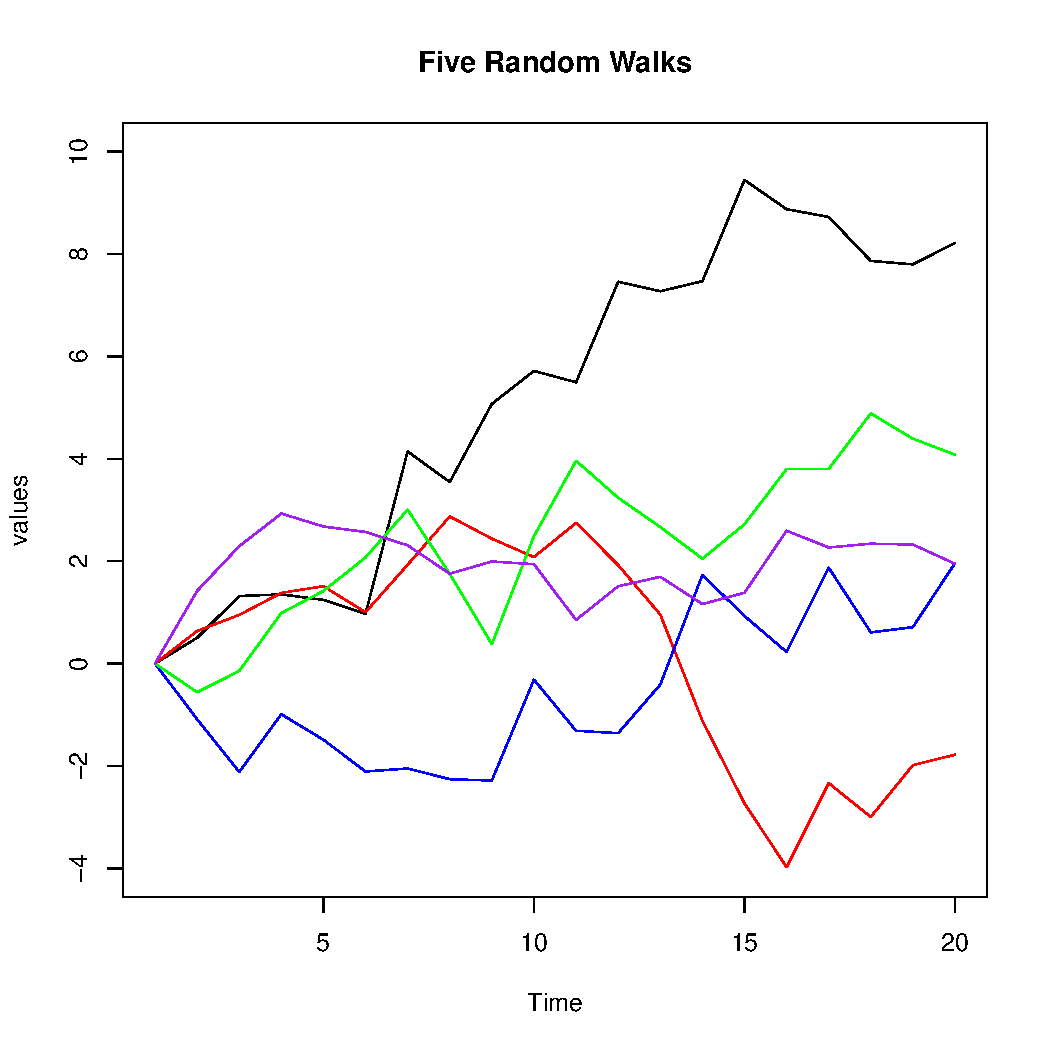
\includegraphics[width=100mm, height=60mm]{randomwalk.pdf}

Any comments?

\end{frame}

\begin{frame}
\frametitle{Random Walk Model}
It is interesting to note that while random walks consist of a
dependent sequence of random variables, it may be easily
transformed into an independent sequence by looking at the
sequence of ``differences''
 \begin{equation}
\nabla x_t=x_{t}-x_{t-1},
 \end{equation}
where $t=1,...,n-1$.
\end{frame}

\section{Autoregressive Models}
\frame{\tableofcontents[currentsection]}

\begin{frame}
\frametitle{Autoregressive Models}

A class of models closely related to the random walk are the
\textbf{autoregressive  models (AR)}.  An autoregressive model is defined so that the
current location is a \textbf{linear combination} of previous locations
plus a random term (Gaussian white noise).
\begin{equation}\label{eq:AR}
x_t=\phi_1 x_{t-1} + \phi_2 x_{t-2}+...+ \phi_p x_{t-p}+w_t.
\end{equation}
This is an AR(p) model. \\
\vspace{5mm}
\textbf{Question:} Under what condition(s) is the random walk a special case of an AR model?

\end{frame}

\section{Moving Average Models}
\frame{\tableofcontents[currentsection]}

\begin{frame}
\frametitle{Moving Average Models}

There is another family of models known as \textbf{moving average
(MA) models}. One way to think about these models is to take a
sliding window and take a weighted average of a white noise
process for everything in the window.  So, start with a white
noise process, $w_1,...,w_n, ...$.  Then a moving average is of
the following form
\begin{equation}\label{eq:MA}
x_t=w_t +\theta_1 w_{t-1}+...+\theta_q w_{t-q}.
\end{equation}
This is an MA(q) model.

\end{frame}

\section{Mean Function}
\frame{\tableofcontents[currentsection]}

\begin{frame}
\frametitle{Mean Function}

The \textbf{mean function} is defined as
\begin{equation}
\mu_t=E(x_t).
\end{equation}
Some properties of expectation:
\vspace{40mm}

\end{frame}

\begin{frame}
\frametitle{Mean Function}

\textbf{Question:} Derive the mean function of a random walk with drift.

\vspace{50mm}

\end{frame}

\begin{frame}
\frametitle{Mean Function}

\textbf{Question:} Derive the mean function of an MA(q) model.

\vspace{50mm}

\end{frame}

\section{Measures of Dependence}
\frame{\tableofcontents[currentsection]}

\begin{frame}
\frametitle{Variance and Covariance}

Recall the definition of \textbf{variance} for a random variable $X$:

\begin{eqnarray}
\mbox{Var}(X) &=& \mbox{E}[(X-\mbox{E}X)^2] \nonumber \\
              &=& \mbox{E}(X^2) - \left(\mbox{E}X\right)^2.
\end{eqnarray}

The \textbf{covariance} for two random variables, $X$ and $Y$:

\begin{equation}
\mbox{Cov}(X,Y)=\mbox{E}[(X-\mbox{E}X)(Y-\mbox{E}Y)].
\end{equation}

The \textbf{correlation} is:

\begin{equation}
\mbox{Corr}(X,Y) = \rho(X,Y) = \frac{\mbox{Cov}(X,Y)}{\sqrt{\mbox{Var}(X)\mbox{Var}(Y)}}.
\end{equation}

\end{frame}

\begin{frame}
\frametitle{Variance and Covariance}
Some properties of variance and covariance:

\vspace{50mm}

\end{frame}

\begin{frame}
\frametitle{Uncorrelated RVs}

Two random variables $X$ and $Y$ are uncorrelated when $\rho(X,Y) = 0$. This implies that

\vspace{40mm}

\end{frame}

\begin{frame}
\frametitle{Uncorrelated RVs are not Independent}

Two random variables $X$ and $Y$ are independent when their joint density is the product of their marginal densities.

\vspace{40mm}

\end{frame}

\begin{frame}
\frametitle{Uncorrelated RVs are not Independent}

If $X$ and $Y$ are independent, then they are also uncorrelated.


\vspace{50mm}

\end{frame}

\begin{frame}
\frametitle{Uncorrelated RVs are not Independent}

However, if $X$ and $Y$ are uncorrelated, they can still be dependent.

\vspace{50mm}

\end{frame}


\begin{frame}
\frametitle{Autocovariance Function}

A common feature of time series is that the observations are dependent. The \textbf{autocovariance function} is defined
as
\begin{equation} \label{eq:autocovariance}
\gamma(s,t)=E[(x_s-\mu_s)(x_t-\mu_t)].
\end{equation}
So, this is simply the covariance between $x_s$ and $x_t$
evaluated at  all combinations.  Covariance measures the
strength of the \textbf{linear dependence} between random variables.  A
covariance that is small for $s,t$ close together generally
implies random variables that are closer to white noise.
Smoother series tend to have a large autocovariance even for
$s$ and $t$ which are far apart.

\end{frame}

\begin{frame}
\frametitle{Autocovariance Function}


{\bf Question:} Find the autocovariance function for the random
walk model.
\vspace{50mm}

\end{frame}

\begin{frame}
\frametitle{Autocovariance Function}

\textbf{Question:} Find the autocovariance function for the MA(2) model.
\vspace{50mm}

\end{frame}

\begin{frame}
\frametitle{Autocorrelation Function}


We also consider the \textbf{autocorrelation function} (ACF) in addition to autocovariance.  The definition is natural and is given by

\begin{equation} \label{eq:acf}
\rho(s,t)=\frac{\gamma(s,t)}{\sqrt{\gamma(s,s) \gamma(t,t)}}
\end{equation}

We will be using the ACF (\ref{eq:acf}) often. The reasons why will become apparent after we discuss \textbf{stationary time series}.

\end{frame}


\end{document} 